%%%%%%%%%%%%%%%%%%%%%%%%%%%%%%%%%%%%%%%%%%%%%%%%%%%%%%%%%%%%%%%%%%%%%%%%%%%%%%%%
%% IEEE SMC 2026 submission -- letter paper, 10pt, conference class.
%% Template: ieeeconf.cls (IEEE Conference Paper Template, LaTeX).
%%%%%%%%%%%%%%%%%%%%%%%%%%%%%%%%%%%%%%%%%%%%%%%%%%%%%%%%%%%%%%%%%%%%%%%%%%%%%%%%
\documentclass[letterpaper, 10 pt, conference]{ieeeconf}
\IEEEoverridecommandlockouts
\overrideIEEEmargins

\usepackage{cite}
\usepackage{graphicx}
\usepackage{booktabs}
\usepackage{multirow}
\usepackage{array}
\usepackage{url}
\usepackage{amsmath}
\usepackage{amssymb}
\usepackage{xcolor}
\usepackage{adjustbox}

\title{\LARGE \bf
MARTC: Multi-Agent Retrieval with \\
Task-State Control
}

\author{Yanlai Wu, Xu Du, Wendong Xiao, and Ying Tang, Fellow, IEEE%
\thanks{Yanlai Wu and Ying Tang are with the Department of Electrical and Computer Engineering, Rowan University, Glassboro, NJ 08028 USA (e-mail: wuyanl37@rowan.edu; tang@rowan.edu). Ying Tang is the corresponding author.}%
\thanks{Xu Du is with Montclair State University (e-mail: dux3@mail.montclair.edu).}%
\thanks{Wendong Xiao is with the School of Automation and Electrical Engineering, University of Science and Technology Beijing, Beijing 100083, P. R. China (e-mail: wdxiao@ustb.edu.cn).}%
}

\begin{document}
\maketitle
\thispagestyle{empty}
\pagestyle{empty}
\setlength{\parskip}{0pt}
\setlength{\textfloatsep}{6pt plus 1pt minus 2pt}
\setlength{\dbltextfloatsep}{6pt plus 1pt minus 2pt}
\setlength{\floatsep}{5pt plus 1pt minus 1pt}
\setlength{\dblfloatsep}{5pt plus 1pt minus 1pt}

\begin{abstract}
Large language models can generate fluent responses, but specialized assistance such as tutoring requires grounding in instructional materials, visible task state, and explicit answer criteria. Classical retrieval-augmented generation (RAG) usually treats grounding as a fixed retrieve-then-read step. This control flow is rigid when the same surface question requires different materials, response structure, or evaluation criteria across situations. We propose \textsc{MARTC} (Multi-Agent Retrieval with Task-State Control), a training-free framework that treats RAG as structured prompt construction rather than query-only passage lookup. A supervisory router selects the dominant context requirement (planning, criteria, adaptation, or instructional materials) and decides whether retrieval should run; LLM-backed specialists then prepare labeled context blocks for a fixed generator and one bounded critique/revision pass. On two educational benchmarks, under matched backbone, corpus, reranker, and response cap, \textsc{MARTC} improves rubric- and teaching-point-oriented automatic metrics and reduces token use in most settings. Latency improves on EduBench and for the 27B TutorEval run, but not for the 4B TutorEval run. These results validate context assembly automatically; human pedagogical evaluation remains future work.
\end{abstract}

\section{INTRODUCTION}
Large language models (LLMs) are increasingly used as specialized assistants because they can generate explanations, diagnose errors, and provide feedback. However, useful assistance cannot rely only on parametric knowledge. Knowledge-grounded dialogue has long shown the value of external instructional materials~\cite{dinan2019wizard}; many assistance settings require grounding in curated resources, user-visible context, task history, and evaluation criteria to avoid fluent but misaligned guidance. Educational tutoring is a concrete and demanding instance of this problem: a tutor must coordinate course materials, worked examples, rubrics, learner-visible context, and dialogue history~\cite{chevalier2024sciencetutors,liu2026agenttutor}.

Classical retrieval-augmented generation (RAG) has therefore become the default grounding mechanism~\cite{lewis2020rag}. In classical RAG, the query is embedded, the top-$k$ most similar passages are retrieved, and the LLM generates a response conditioned on those passages. Thus, relevance depends heavily on retrieval quality and query representation~\cite{thakur2021beir}.

Specialized assistance, such as tutoring, is more complex than factual question answering. The appropriate response may depend on user background, current goal, task history, prior confusion, and evaluation criteria. We call all information available before generation---the learner profile, task, dialogue, rubric, and inline context---the \emph{task state}. \emph{Task-state control} is the explicit routing and prompt-assembly mechanism that decides which of these visible constraints should dominate the response. A response must therefore be grounded not only in topically relevant instructional materials but also in the user's state and task-specific requirements.

Classical RAG can include explicit state text when supplied, but appending user state, dialogue, criteria, and task constraints forces one query embedding to compress topic, level of detail, intent, and response requirements. As constraints grow, search intent can blur. The issue is therefore how a response system should organize constraints before retrieval and generation.

We therefore introduce \textsc{MARTC} for LLM-based tutoring. Its central contribution is a bounded, training-free context controller rather than a new retriever, generator, or open-ended agent loop. By \emph{structured prompt construction}, we mean separating search intent, learner-state diagnosis, criteria interpretation, and retrieved evidence into labeled blocks before one generator call. A cue-based router selects a prompt-priority regime and retrieval gate; specialist agents fill the corresponding blocks; and one critic checks the draft against the same brief. This design keeps state and criteria available without forcing them into one retrieval embedding.

\noindent\textbf{Contributions.} (i) We introduce a transparent controller that combines cue-based task-state routing, specialist prompt construction, and conditional retrieval. (ii) We specify a bounded contract: parallel specialists return structured records, a fixed generator writes one draft, and a critic performs at most one revision. (iii) We validate the controller against Classical and Agentic RAG under paired infrastructure and report quality and resource trade-offs across two backbones.

\section{RELATED WORK}

\noindent\textbf{RAG controllers.} Classical RAG fixes retrieval as the first controller~\cite{lewis2020rag}. Self-RAG learns reflection tokens for retrieval and critique~\cite{asai2024selfrag}; CRAG evaluates retrieved documents and may expand to web search~\cite{yan2024crag}; Adaptive-RAG learns to choose a reasoning strategy from question complexity~\cite{jeong2024adaptiverag}; and TARG applies a training-free retrieve-or-skip gate to a no-context draft~\cite{wang2026targ}. These methods control whether, when, or how retrieval is corrected. MARTC instead controls which visible task constraint is represented before retrieval and keeps state and criteria in separate generator blocks. RAG diagnostics identify retrieval and generation failures but do not provide this controller~\cite{ru2024ragchecker}.

\noindent\textbf{Agentic retrieval.} ReAct, AutoGen, CAMEL, and MetaGPT interleave actions or coordinate roles for broad task execution~\cite{yao2023react,wu2024autogen,li2023camel,hong2024metagpt}. MA-RAG decomposes ambiguous and multi-hop QA into an iterative answer-solving chain~\cite{nguyen2025marag}. MARTC differs in scope: its agents are bounded context producers, not autonomous answer solvers, and all branches converge on the same generator and one critique pass. Agentic RAG in our experiments retains the specialist scaffold but removes MARTC's prompt-priority regime and retrieval gate, isolating whether coordination alone explains the result.

\noindent\textbf{Educational agents and evaluation.} AgentTutor maintains memory and adapts teaching strategy across turns~\cite{liu2026agenttutor}; tutoring benchmarks assess pedagogical response properties~\cite{maurya2025aitutoreval,chevalier2024sciencetutors,xu2025edubench,macina2025mathtutorbench,srinivasa2025tutorbench}. MARTC is not a complete tutoring policy: it isolates context construction under a fixed generator so memory, dialogue policy, and teaching strategy do not absorb the retrieval effect.

\section{METHODOLOGY}
\label{sec:methodology}

Specialized assistance must determine what the user is asking, what state is visible, what criteria apply, and whether external materials are needed. These decisions make context construction a distinct stage before generation. \textsc{MARTC} coordinates that stage through input normalization, supervisor routing, and specialist agents (Fig.~\ref{fig:martc_framework}); Algorithm~1 summarizes inference.

\begin{figure*}[t]
\centering
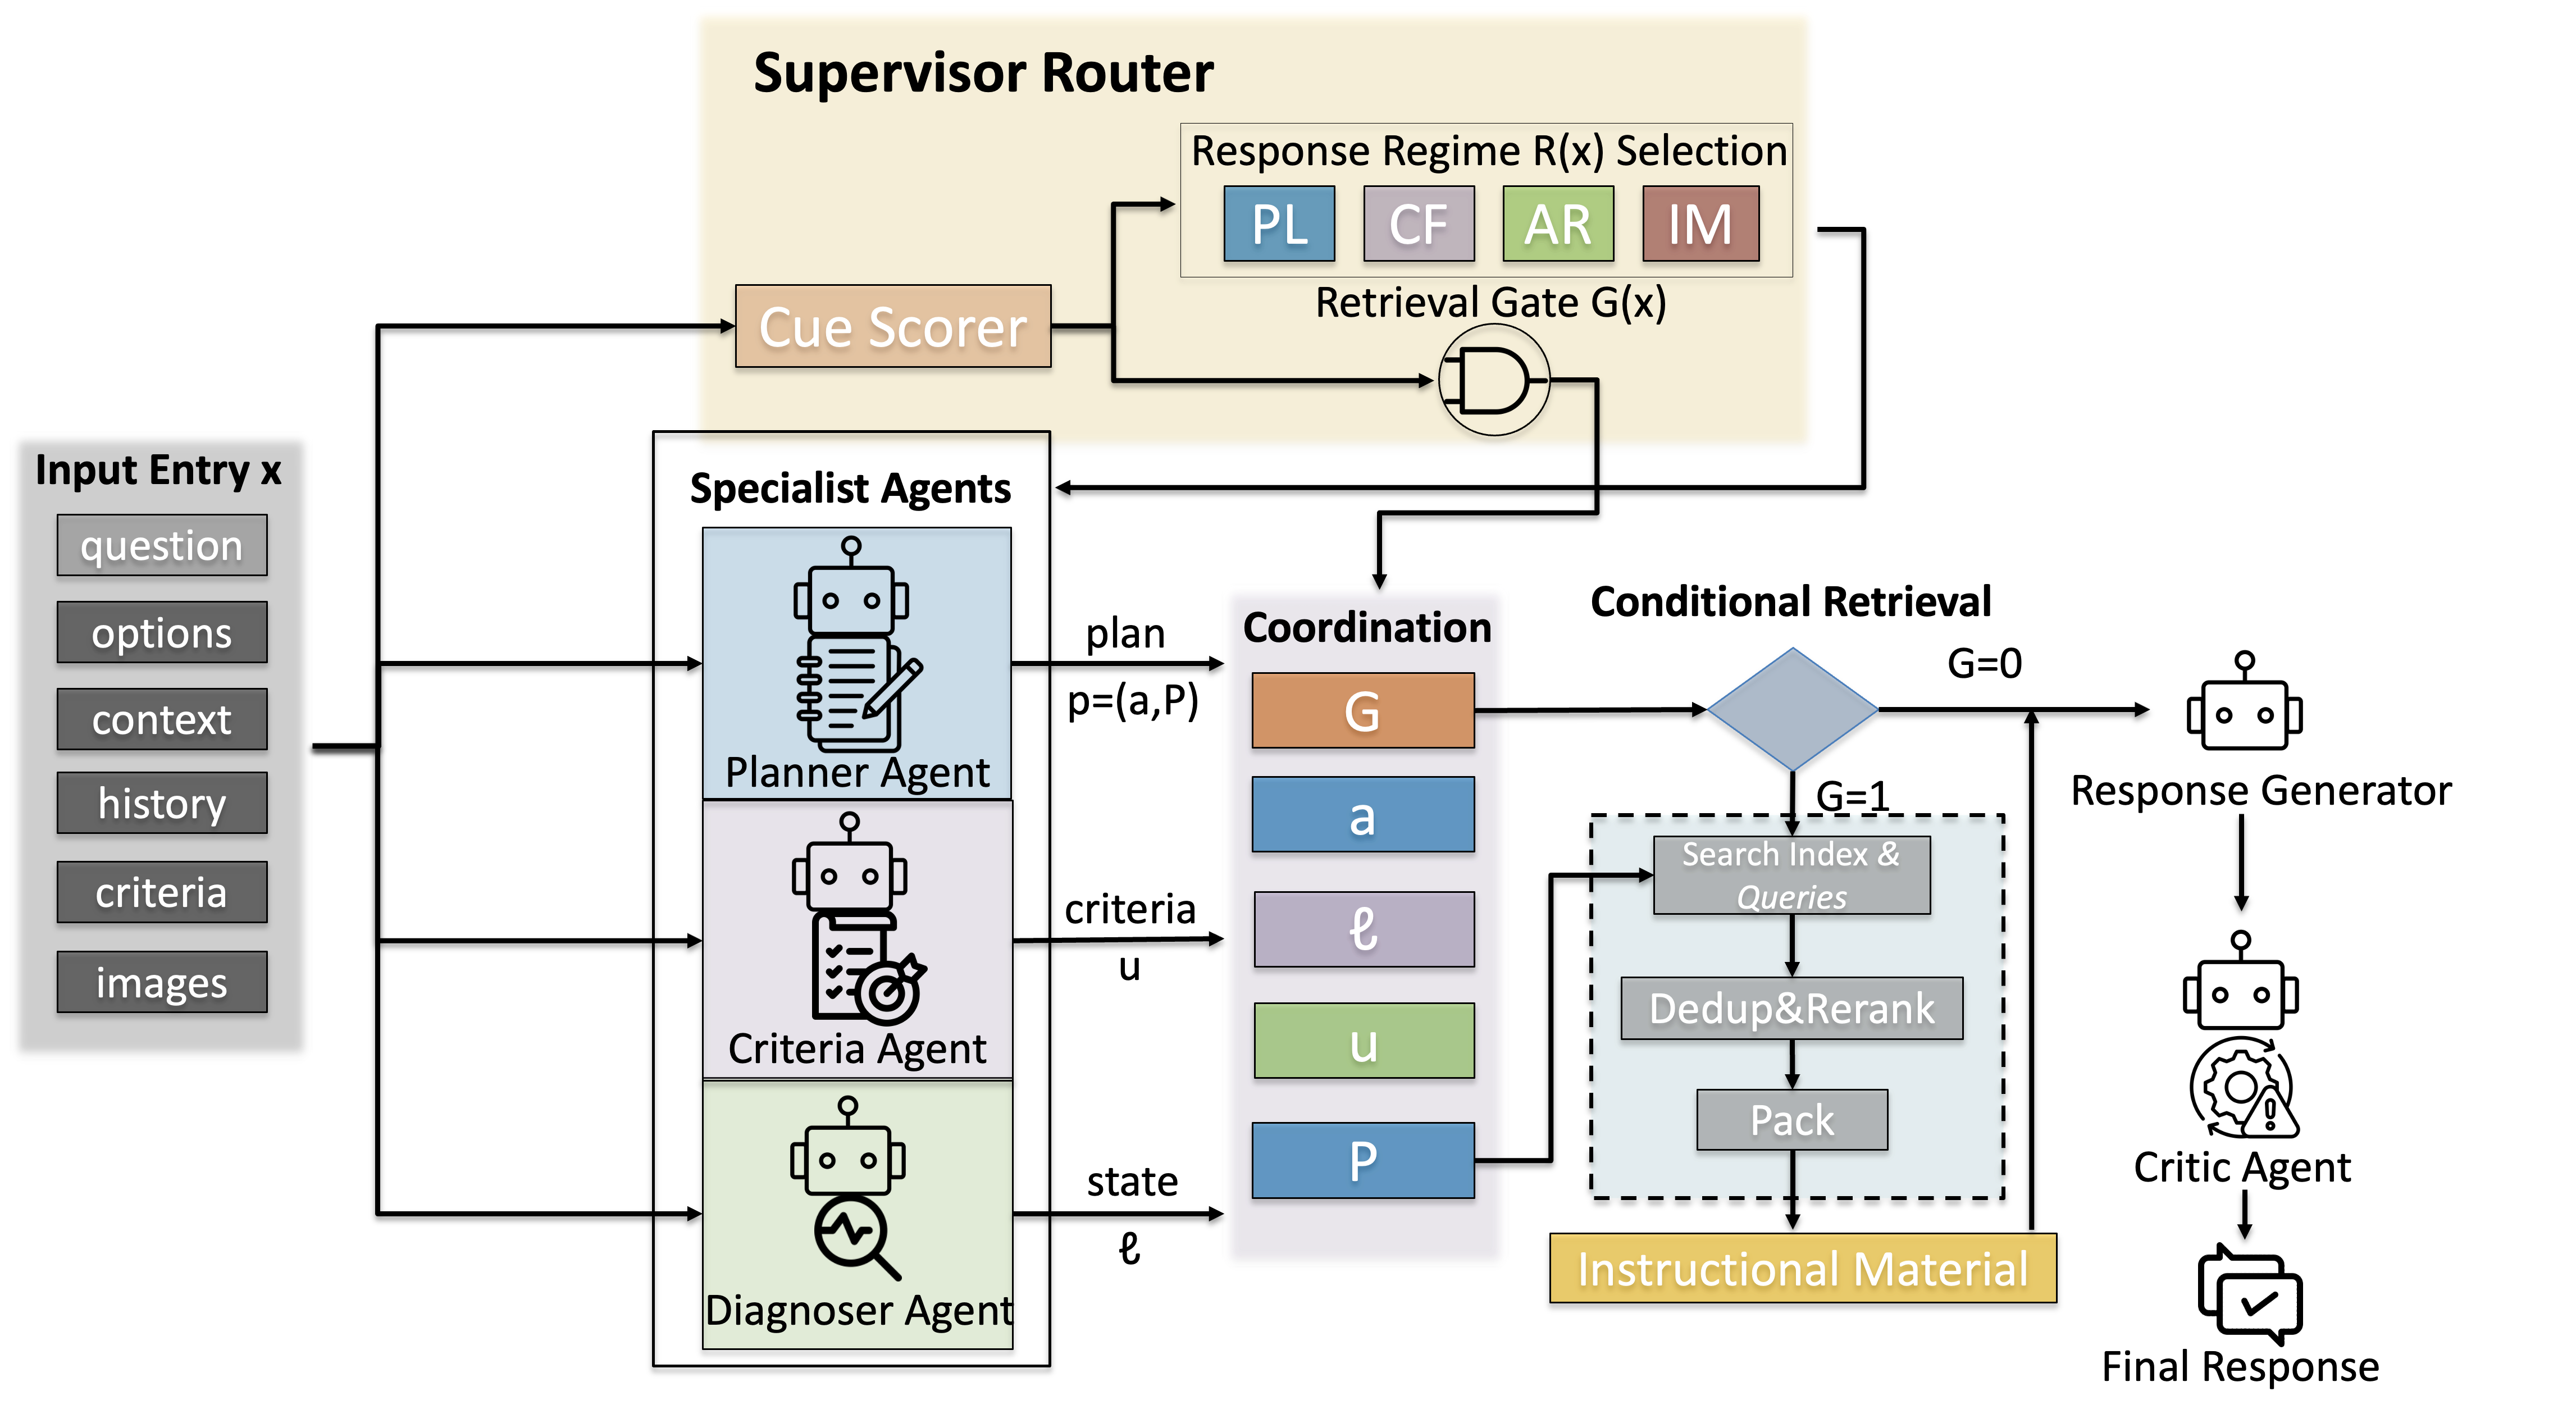
\includegraphics[width=0.96\textwidth]{figures/marlet_main_final.png}
\caption{Main framework of \textsc{MARTC}. A normalized entry $x=(q,o,c,h,r,v)$ is scored by the supervisor router, which selects the response regime $R(x)\in\{\mathrm{PL},\mathrm{CF},\mathrm{AR},\mathrm{IM}\}$ and retrieval gate $G(x)$. LLM-based specialist agents then produce structured prompt blocks: planner strategy $a$ and search queries $P$, criteria summary $u$, and learner-state summary $\ell$. The coordinator merges these blocks with retrieved snippets into instructional-material bundle $D$ when $G(x)=1$, then sends one augmented prompt to the generator and critic.}
\label{fig:martc_framework}
\end{figure*}

\subsection{Input Normalization}

\textsc{MARTC} first converts each request into one normalized input entry:
\begin{equation}
x=(q,o,c,h,r,v).
\end{equation}
The entry contains only information visible before generation. Here, $q$ is the question or task; $o$ is any answer-option set; $c$ is inline context already provided with the request; $h$ is recent interaction history; $r$ is explicit criteria such as a rubric or required feedback points; and $v$ stores images when present. Any field may be empty. This normalization step is deliberately separated from agent outputs: it only standardizes heterogeneous inputs so the router and specialist agents receive the same interface. This prevents topic, state, criteria, and instructional-material needs from being compressed into a single long retrieval query~\cite{liu2026agenttutor,borchers2025adaptivity}.

\subsection{Supervisor Routing}
The supervisory router is responsible for mapping each input sample to a response regime and activating the corresponding specialist agents. Given an input sample, the router examines the visible question, optional context, dialogue history, learner-state information, rubric or criteria text, and task metadata. It then estimates four types of context need: planning, criteria feedback, learner-state adaptation, and instructional-material support.

These needs correspond to four regimes. Planning (PL) is selected when the response requires an ordered structure, such as step sequencing, lesson planning, or exercise design. Criteria Feedback (CF) is selected when the response must be judged against explicit requirements, such as rubrics, scoring rules, or required feedback fields. Adaptive Response (AR) is selected when the same content should be explained differently depending on visible user state, such as grade level, prior confusion, weak points, or preferred explanation style. Instructional Materials (IM) is selected when the response should be supported by external resources, such as textbook chapters, reference documents, or worked examples.

To make routing transparent and training-free, MARTC uses cue scores rather than a learned classifier. It first constructs
\begin{equation}
b(x)=\mathrm{concat}(q,c,r,h),
\end{equation}
where the four textual fields are normalized and concatenated. Images remain available downstream but are not converted to text. For family $j\in\{\mathrm{im},\mathrm{cr},\mathrm{pl},\mathrm{ad}\}$, let $W_j$ be its cue lexicon and $M_j(x)$ the number of distinct cues occurring in $b(x)$. The score is
\begin{equation}
s_j(x)=\min\left(1,\frac{M_j(x)}{|W_j|}+\delta_j(x)\right),
\end{equation}
where each phrase contributes at most once. The exact released lexicons are: IM=\{cite, citation, source, evidence, supporting facts, reference, grounded, retrieval, document, chapter, lecture, verification\}; CF=\{rubric, criterion, criteria, score, feedback, comment\}; PL=\{plan, sequence, schedule, workflow, roadmap, steps, next steps, lesson, curriculum, study schedule, exercise plan\}; and AR=\{user, profile, beginner, expert, personalize, adapt, confused, attempted, hint, misconception, student, explain, teach, tutor\}. The explicit adjustments are $+0.20$ to CF when a rubric is present, up to $+0.50$ to AR from dialogue length, $+0.08$ to IM for inline context, and $+0.05$ to IM for an image.

The fixed thresholds prevent incidental matches from changing behavior. We use $\tau_{\rm mid}=0.35$ for CF, AR, and retrieval and $\tau_{\rm plan}=0.42$ for PL, whose selection changes response structure. The same values are used for both benchmarks and backbones. A gate sweep over $[0.30,0.55]$ left aggregate quality unchanged over $[0.30,0.45]$, so the reported conclusion does not depend on the exact value $0.35$ within that interval.

Based on these cues and thresholds, the supervisor assigns the response regime as follows:
\begin{equation}
R(x)=
\begin{cases}
\mathrm{PL}, & s_{\rm pl}\ge s_{\rm cr},\ s_{\rm pl}\ge s_{\rm ad},\ s_{\rm pl}\ge\tau_{\rm plan},\\
\mathrm{CF}, & s_{\rm cr}\ge s_{\rm ad},\ s_{\rm cr}\ge\tau_{\rm mid},\\
\mathrm{AR}, & s_{\rm ad}\ge \tau_{\rm mid},\\
\mathrm{IM}, & \mathrm{otherwise}.
\end{cases}
\end{equation}
In addition to selecting the prompt-priority regime, the supervisor makes a binary retrieval decision~\cite{asai2024selfrag,jeong2024adaptiverag,wang2026targ}:
\begin{equation}
G(x)=
\begin{cases}
1, & s_{\rm im}\ge \tau_{\rm mid}\ \mathrm{or}\ R(x)=\mathrm{IM},\\
0, & \mathrm{otherwise}.
\end{cases}
\end{equation}
Thus, retrieval runs when material cues are strong or IM is the default regime. Routing is auditable but lexical: a rubric-bearing grading request without stronger planning/adaptation cues routes to CF, while several dialogue turns showing prior confusion can route to AR; conversely, quoted syllabus language containing ``plan,'' ``schedule,'' ``roadmap,'' and ``next steps'' can spuriously trigger PL. This false-positive mode motivates learned calibration and routing-error analysis in future work.

\subsection{Specialist Agents and Coordination}
After routing, the planner, criteria agent, and diagnoser construct a response brief in parallel. Each independently returns a structured record, and the coordinator merges the records into one prompt.

The planner returns $p=(a,P)$, where $a$ is a response strategy and $P$ is a short list of scoped retrieval queries. The criteria agent returns $u$, summarizing rubrics, grading rules, required fields, or default quality criteria. The diagnoser returns $\ell$, summarizing level, goals, misconceptions, prior confusion, or preferred style. MARTC also maintains bundle $D$ for retrieved snippets. Only answer $y$ is user-facing; all other slots are prompt context.

After generation, the critic performs one bounded pass over the brief, materials, and draft to check material use, criteria coverage, and learner-state alignment. It revises once if needed; otherwise it returns the draft.

Each regime changes the brief. PL gives the planner's structure priority; CF foregrounds evaluation criteria; AR foregrounds $\ell$ for tone, depth, and scaffolding; and IM uses $P$ to retrieve materials. The final prompt combines the original task, regime, $p$, $\ell$, $u$, and $D$ when available. This is the structured prompt-construction contract that distinguishes MARTC from an open-ended multi-agent solving chain.

\begin{center}
\centering
\scriptsize
\setlength{\tabcolsep}{0pt}
\renewcommand{\arraystretch}{0.96}
\begin{tabular}{@{}r@{\hspace{0.45em}}p{0.89\columnwidth}@{}}
\toprule
\multicolumn{2}{@{}l@{}}{\textbf{Algorithm 1: \textsc{MARTC} Inference Process}}\\
\midrule
\multicolumn{2}{@{}p{0.96\columnwidth}@{}}{\textbf{Require:} entry $x=(q,o,c,h,r,v)$, index $\mathcal{I}$, thresholds $(\tau_{\rm mid},\tau_{\rm plan})$.}\\
\multicolumn{2}{@{}p{0.96\columnwidth}@{}}{\textbf{Return:} answer $y$ and internal fields $(R,G,p,\ell,u,D)$.}\\
\midrule
1: & $b\leftarrow \mathrm{concat}(q,c,r,h)$; $(s_{\rm im},s_{\rm cr},s_{\rm pl},s_{\rm ad})\leftarrow\mathrm{CueScores}(b)$\\
2: & $R\leftarrow R(x)$ using Eq. (4); $G\leftarrow G(x)$ using Eq. (5)\\
3: & \textbf{parallel do}\\
4: & \quad $p=(a,P)\leftarrow\mathrm{Planner}(x,R,G)$\\
5: & \quad $\ell\leftarrow\mathrm{Diagnoser}(q,h)$\\
6: & \quad \textbf{if} $r\ne\emptyset$ or $R=\mathrm{CF}$ \textbf{then} $u\leftarrow\mathrm{Criteria}(x,R)$\\
7: & \quad \textbf{else} $u\leftarrow\mathrm{DefaultCriteria}()$\\
8: & \quad \textbf{end if}\\
9: & \textbf{end parallel}\\
10: & $D\leftarrow\emptyset$\\
11: & \textbf{if} $G=1$ \textbf{then}\\
12: & \quad $D\leftarrow \mathrm{Pack}(\mathrm{Rerank}(\mathrm{Dedup}(\mathrm{Search}(\mathcal{I},P)),q))$\\
13: & \textbf{end if}\\
14: & $y_0\leftarrow A_{\rm gen}(\mathrm{Prompt}(q,o,h,p,\ell,u,D,c))$\\
15: & $y\leftarrow\mathrm{CriticOnce}(y_0,q,h,p,\ell,u,D,r)$\\
16: & \textbf{return} $y,(R,G,p,\ell,u,D)$\\
\bottomrule
\end{tabular}
\end{center}

\section{VALIDATION EXPERIMENTS}
\label{sec:results}

We validate the framework on two public educational benchmarks used as tutoring-focused stress tests. TutorEval~\cite{chevalier2024sciencetutors} pairs science tutoring questions with long STEM chapters and teaching key points; EduBench~\cite{xu2025edubench} covers diverse educational scenarios with prompts, metadata, and reference model predictions that our adapter converts into score and rubric supervision.

The primary validation compares context-assembly methods under matched infrastructure for both \textsc{Qwen3.5-4B} and \textsc{Qwen3.5-27B-FP8}, which checks whether the trends hold across backbone size. Classical RAG retrieves first from the raw standardized prompt; visible learner profile, student answer, dialogue, and criteria text remain available to its generator prompt, so the baseline is not deprived of task context. Its limitation is controller order: retrieval happens before specialist summaries can shape search. Agentic RAG uses the same specialist-coordination scaffold without MARTC's task-state retrieval control, so it tests whether agent coordination alone explains the gains. \textsc{MARTC} keeps the same backbone and corpus resources, then adds supervisory routing, conditional retrieval, and bounded context assembly. We report quality and cost together because only context construction changes.

\subsection{Implementation Details}

All controllers use the same Python framework, corpus, hybrid text index, reranker, generator, critic, cache policy, and metric code; only context assembly differs. Specialists and the generator use the same configured backbone, with deterministic fallbacks only for unavailable or malformed LLM output. MARTC permits bounded local observations and corpus search, without network, file mutation, or open-ended shell tools. SGLang serves the endpoints~\cite{zheng2024sglang}. Exact model-response caching requires an identical full payload and is recorded in artifacts; latency is therefore cache-aware served wall time, not a cold-start benchmark.

Runs use \textsc{Qwen3.5-4B} and \textsc{Qwen3.5-27B-FP8}~\cite{qwen35}, reasoning budget 512, generation temperature 0.15, specialist JSON temperature 0.0, and response cap 900 on \texttt{benwulab-Lambda-Vector} with two NVIDIA RTX 6000 Ada GPUs. Retrieval packs up to four snippets from at most three planner queries under a 6000-character context cap. For each backbone, TutorEval uses $n{=}400$ paired samples; EduBench uses $n{=}328$ unique paired rows after duplicate public IDs in the 400-example slice are collapsed.

All quality scores are automatic proxies, not official human grades. Token-F1 is token-overlap precision/recall F1 against the reference. Rubric coverage averages exact or content-bearing partial matches to required criteria. Tutor-hit assigns full, partial, or zero credit to expert teaching points. EB12D averages 12 normalized checks over scenario adaptation, factual/reasoning behavior, and pedagogical application; EduAlign measures extracted-score agreement with benchmark consensus. Latency is served seconds per sample, and tokens include prompt and completion tokens. These metrics separate overlap, criteria fulfillment, instructional-material use, and resource cost~\cite{ru2024ragchecker}, but do not directly measure learning gains.

\subsection{Framework Validation}

Tables~\ref{tab:validation_summary} and~\ref{tab:validation_27b} compare Classical RAG, Agentic RAG, and \textsc{MARTC}. Agentic RAG tests whether specialist coordination alone explains the gains. Significance markers compare paired MARTC--RAG samples using 10,000 paired permutations; 95\% intervals use 2,000 paired bootstrap resamples.

\begin{table}[t]
\caption{4B quality and resource summary with Agentic comparison.}
\label{tab:validation_summary}
\centering
\scriptsize
\setlength{\tabcolsep}{1.7pt}
\renewcommand{\arraystretch}{0.96}
\begin{tabular}{@{}llrrrr@{}}
\toprule
Data & Metric & RAG & Agentic & MARTC & $\Delta$ \\
\midrule
\multirow{5}{*}{TutorEval} & Token-F1 & 0.112 & 0.090 & \textbf{0.115} & $+0.004^{\star}$ \\
& Tutor hit & 0.938 & 0.932 & \textbf{0.957} & $+0.019^{\star\star}$ \\
& Rubric & 0.919 & 0.907 & \textbf{0.944} & $+0.026^{\star\star}$ \\
& Latency (s) & 31.90 & \textbf{31.05} & 39.11 & $+7.21$ \\
& Tokens & 3975 & 5959 & \textbf{3490} & $-484^{\star\star\star}$ \\
\midrule
\multirow{5}{*}{EduBench} & EB12D & 0.367 & \textbf{0.398} & \textbf{0.398} & $+0.031^{\star\star\star}$ \\
& Rubric & 0.705 & \textbf{0.891} & \textbf{0.891} & $+0.186^{\star\star\star}$ \\
& EduAlign & \textbf{0.166} & 0.130 & 0.126 & $-0.040^{\star\star}$ \\
& Latency (s) & 19.83 & 23.73 & \textbf{13.90} & $-5.92^{\star\star\star}$ \\
& Tokens & 4020 & 5224 & \textbf{2226} & $-1794^{\star\star\star}$ \\
\bottomrule
\end{tabular}
\begin{minipage}{\columnwidth}\scriptsize\vspace{0.1em}Agentic omits MARTC's task-state retrieval control. Bold is best among the three methods; lower is better for latency/tokens. $\Delta$ and significance compare paired MARTC--RAG only: $^{\star\star\star}p{<}10^{-4}$, $^{\star\star}p{<}0.01$, $^{\star}p{<}0.05$.\end{minipage}
\end{table}

\begin{table}[t]
\caption{27B quality and resource summary with Agentic comparison.}
\label{tab:validation_27b}
\centering
\footnotesize
\setlength{\tabcolsep}{2.2pt}
\renewcommand{\arraystretch}{0.90}
\begin{tabular}{llrrrr}
\toprule
Data & Metric & RAG & Agentic & MARTC & $\Delta$ \\
\midrule
\multirow{5}{*}{TutorEval} & Token-F1 & 0.264 & 0.270 & \textbf{0.272} & $+0.008^{\star}$ \\
& Tutor hit & 0.897 & 0.902 & \textbf{0.918} & $+0.021^{\star}$ \\
& Rubric & 0.861 & 0.873 & \textbf{0.891} & $+0.030^{\star}$ \\
& Latency (s) & 41.47 & 48.31 & \textbf{40.65} & $-0.82^{\star\star}$ \\
& Tokens & \textbf{6681} & 7200 & 6730 & $+49$ \\
\midrule
\multirow{5}{*}{EduBench} & EB12D & 0.355 & 0.389 & \textbf{0.425} & $+0.070^{\star\star\star}$ \\
& Rubric & 0.634 & 0.748 & \textbf{0.769} & $+0.135^{\star\star\star}$ \\
& EduAlign & \textbf{0.541} & 0.511 & 0.526 & $-0.015$ \\
& Latency (s) & 41.91 & 50.21 & \textbf{32.09} & $-9.81^{\star\star\star}$ \\
& Tokens & 6105 & 5829 & \textbf{3717} & $-2388^{\star\star\star}$ \\
\bottomrule
\end{tabular}
\begin{minipage}{\columnwidth}\scriptsize\vspace{0.1em}Agentic omits MARTC's task-state retrieval control. Bold is best among the three methods; lower is better for latency/tokens. $\Delta$ and significance compare paired MARTC--RAG only: $^{\star\star\star}p{<}10^{-4}$, $^{\star\star}p{<}0.01$, $^{\star}p{<}0.05$.\end{minipage}
\end{table}

\subsection{Discussion}

TutorEval gains in tutor-hit and rubric coverage suggest that planner, criteria, and diagnoser slots preserve teaching points and requirements when materials are long. EduBench gains in EB12D and rubric coverage suggest that task-state control helps when requests combine scenario, answer constraints, and feedback style. Agentic RAG is competitive on some quality metrics but often uses more tokens and time because its specialist outputs are not filtered through MARTC's gate and regime.

EduAlign should be interpreted narrowly because it measures agreement with extracted consensus scores, whereas MARTC constructs criteria-aware responses. The resource results also show a trade-off: scoped queries and gating usually reduce tokens and 27B latency, but 4B TutorEval latency increases by 7.21\,s and 27B TutorEval uses 49 more tokens. MARTC is therefore not a universal lower-cost guarantee.

\subsection{Limitations}

First, automatic proxies do not establish pedagogical helpfulness, trust, affect, or learning gains; no human expert study is reported. Second, the manually specified English cue lexicons can produce lexical false positives, and the gate sweep does not replace labeled routing-accuracy analysis. Third, the benchmarks are English-only and mostly single-turn. Human evaluation, multi-turn outcomes, multilingual calibration, and stronger learned-router baselines are needed before broader tutoring claims.

\section{CONCLUSION}
\label{sec:conclusion}

\textsc{MARTC} reframes grounding as supervised context construction rather than query-only passage lookup. Its contribution is a training-free controller that separates task-state diagnosis, criteria interpretation, planning, and conditional retrieval before a fixed generator. Under paired automatic validation, this organization improves rubric- and teaching-point-oriented metrics while often reducing resource use. Human and multi-turn evaluation must determine whether these proxy gains translate into better tutoring.

\section*{ACKNOWLEDGMENT}
The authors gratefully acknowledge the support of Google Academic Research Awards.

\bibliographystyle{IEEEtran}
\bibliography{references/references}

\end{document}
